\begin{frame}
    \begin{center}
        \textcolor{NJU_purple}{\Large 第三部分} \\[1.5em]
        \textcolor{NJU_purple}{\Huge 模型设计}
    \end{center}
\end{frame}

\begin{frame}{模型设计总体框架}
    \centering
    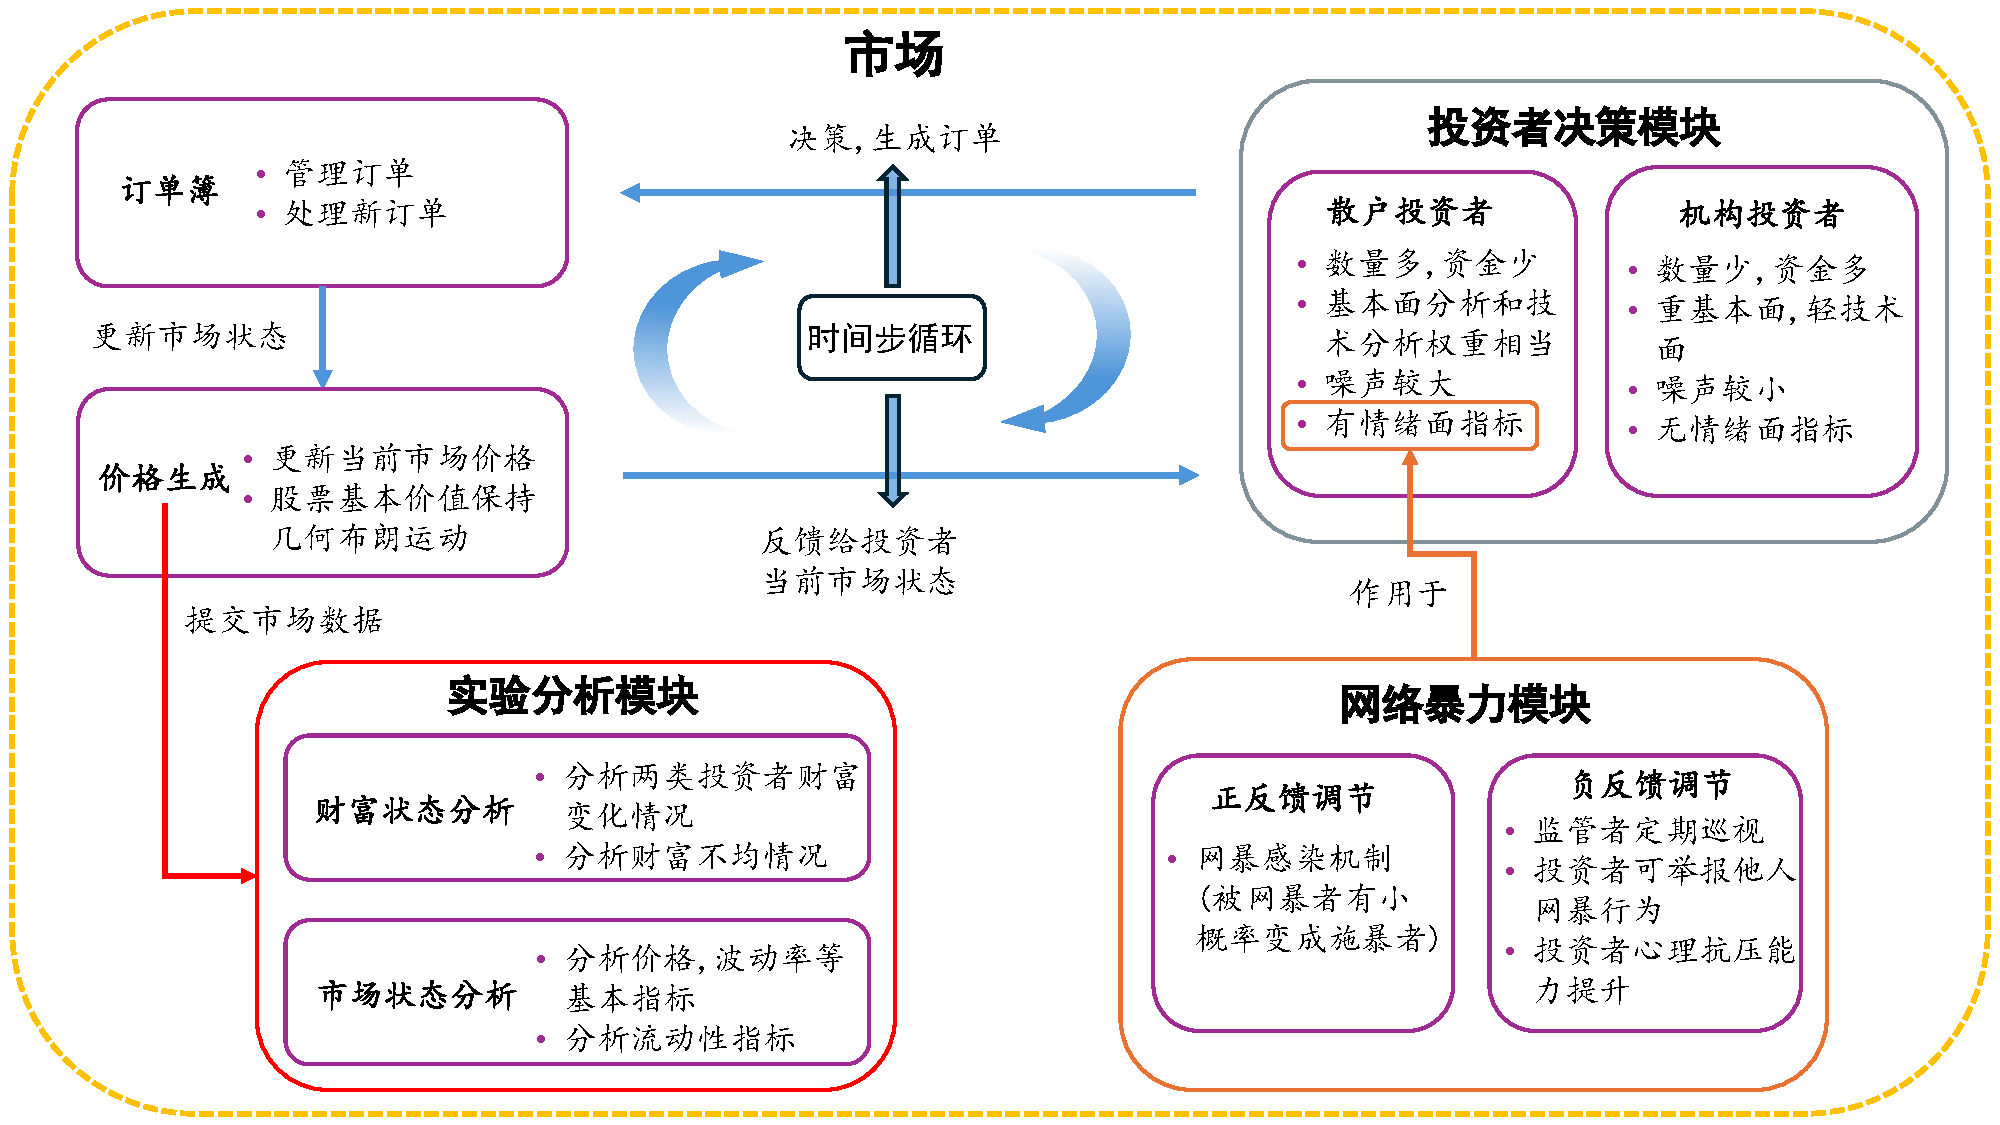
\includegraphics[width=1.0\textwidth]{pic/3-1_structure.pdf}  % 请替换为你的实际图路径
    \end{frame}


\begin{frame}{模型设计——市场结构模块}

    \footnotesize
    \setlength{\parskip}{0.2em}
    \linespread{0.9}
    
    \begin{itemize}
        \item 本研究参照Chiarella 等(2009),在离散时间步的的设定下,模拟了一个订单驱动的股票市场,核心机制为\textbf{连续双边订单簿撮合}。
    
        \item \textbf{订单簿实现机制:}
        \begin{itemize}
            \item 系统同时维护买方与卖方两个限价簿,按价格优先、时间优先排序;
            \item 市价单立即与对手簿最优价撮合,限价单则挂入簿中等待成交;
            \item 支持挂单、撤单、部分成交、打穿多个价位等情形;
            \item 数据结构采用哈希表 + 优先队列(最小堆)组合,支持高频仿真与快照提取。
        \end{itemize}
    
        \item \textbf{市场价格生成规则:}
        \begin{itemize}
            \item 当一笔或多笔市价单成交时,取加权平均成交价作为当期市场交易价格 \( p_t \);
            \item 系统同时记录最优买价 \( b_t^q \) 与最优卖价 \( a_t^q \),用于投资者下单判断;
            \item 市场价格作为投资者预期收益率计算的重要输入。
        \end{itemize}
    
        \item \textbf{基础价格的生成方式:} \\
        市场基础价值 \( p_t^f \) 服从几何布朗运动(GBM)过程,用于模拟基本面价格变化:
        $$
        dp_t^f = \mu p_t^f dt + \sigma p_t^f dW_t
        $$
        其中 \( \mu \) 为漂移项、\( \sigma \) 为波动率、\( W_t \) 为标准布朗运动。
    
        \item \textbf{补充:} Chiarella 等(2009)只支持每个时间步一个投资者进入市场交易。为增强模拟的灵活性,本研究支持交易者执行三种模式:single / partial / all。
    
    \end{itemize}
    
    \end{frame}



\begin{frame}{模型设计——投资者行为模块}
    \vspace{-0.4em}
    \footnotesize
    \setlength{\parskip}{0.2em}
    \linespread{0.9}
    
    \begin{itemize}
        \item 投资者分为散户和机构。机构数量占比较少,初始财富较大,投资逻辑更偏\alert{理性和基本面}。二者根据以下公式决定自己的预期收益率与预期价格:
    \end{itemize}
    
    \vspace{-0.4em}
    
    \[
    \hat{r}_{t,t+\tau^i}^i = 
        \frac{1}{g_1^i + g_2^i + g_e^i + n^i } 
        \left[
        \underbrace{g_1^i \cdot \frac{1}{\tau_f} \ln\left(\frac{p_t^f}{p_t}\right)}_{\text{基本面}} 
        + \underbrace{g_2^i \cdot \bar{r}_t^i}_{\text{技术面}} 
        + \underbrace{g_e^i \cdot \eta_t^i}_{\text{情绪偏差}}
        + \underbrace{n^i \cdot \epsilon_t}_{\text{噪音}} 
        \right]
    \]
    \scriptsize
    注:\(g_1^i, g_2^i, g_e^i, n^i\) 分别为投资者对基本面、技术面、情绪与噪声的关注权重;
    \(p_t^f\) 为基础价值,\(\bar{r}_t^i\) 为平均收益率,\(\eta_t^i\) 为情绪偏差(仅对散户有效),\(\epsilon_t\) 为噪声,\( \tau^i \)为投资者 \(i\) 的视野期, \( \bar{r}_t^i \)为投资者 \(i\) 观察到的近期平均收益率。

    \vspace{-0.4em}
    
    
    \footnotesize

    \begin{itemize}
        \item 计算预期价格后,投资者将其与当前市场最优买卖报价($a_t^q, b_t^q$)进行比对,以确定订单的方向和类型,规则如下:
    \end{itemize}
    
    \vspace{-0.6em}
    \center
    \begin{tabular}{@{} >{\centering\arraybackslash}p{4.5cm} 
        >{\centering\arraybackslash}p{3.5cm} 
        >{\centering\arraybackslash}p{4.5cm} @{}}
        \toprule
        价格区间 & 方向 & 订单类型 \\
        \midrule
        \( p_m < p < a_t^q \) & 买入 & 限价单 \\
        \( a_t^q \le p < p^* \) & 买入 & 市价单 \\
        \( p \approx p^* \) & 不交易 & 无 \\
        \( p^* < p \le b_t^q \) & 卖出 & 市价单 \\
        \( b_t^q < p < p_M \) & 卖出 & 限价单 \\
        \bottomrule
    \end{tabular}

    \begin{itemize}
        \item 订单数量通常通过在账户余额的基础上乘以一个范围内波动的比例系数(如 0.2 到 0.5)生成,对于散户投资者,其交易数量中包含一个噪声项,使得其交易行为更具不确定性,且若该散户处于网络暴力的“被攻击者”状态,其交易数量会受到放大,体现出行为激进化特征。
    \end{itemize}
    
\end{frame}

\begin{frame}{模型设计——网络暴力模块}

\end{frame}

